\begin{figure}[t]

\caption{Neighborhoods in Syntagmatic Graphs}	

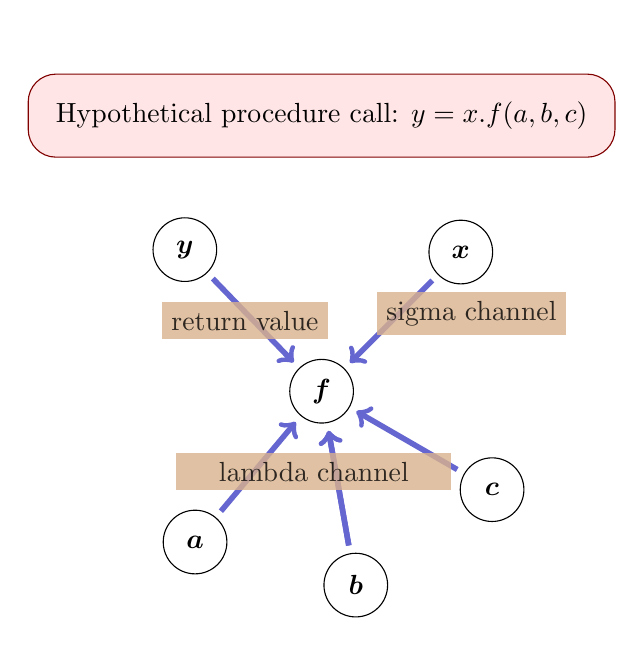
\begin{tikzpicture}

\node (dummy) at (0,1) {};

\node (text) at (0,0) [draw=red!50!black,fill=red!10, inner sep=10pt,
minimum size=25pt,rounded corners = 10pt]{Hypothetical procedure call: $y = x.f(a,b,c)$};

%\pgfmathsetmacro\n{6}
%\pgfmathsetmacro\r{1*(360/\n)}

\node (f) at (0,-3.5) [circle,draw=black, inner sep=0pt,
minimum size=23pt,font=\boldmath]{$f$};

\node (y) at ([shift=({134:25mm})]f) [circle,draw=black, inner sep=0pt,
minimum size=23pt,font=\boldmath]{$y$};

\node (x)  at ([shift=({45:25mm})]f) [circle, draw=black, inner sep=0pt,
minimum size=23pt,font=\boldmath]{$x$};

\node (a)  at ([shift=({230:25mm})]f) [circle, draw=black, inner sep=0pt,
minimum size=23pt,font=\boldmath]{$a$};

\node (b)  at ([shift=({280:25mm})]f) [circle, draw=black, inner sep=0pt,
minimum size=23pt,font=\boldmath]{$b$};

\node (c) at ([shift=({330:25mm})]f) [circle, draw=black, inner sep=0pt,
minimum size=23pt,font=\boldmath]{$c$};

\colorlet{blbl}{blue!70!black}
\draw [line width=2pt, blbl!60, ->, 
shorten <= 1mm, shorten >= 1mm] (a) -- (f); 

\draw [line width=2pt, blbl!60, ->, 
shorten <= 1mm, shorten >= 1mm] (b) -- (f); 

\draw [line width=2pt, blbl!60, ->, 
shorten <= 1mm, shorten >= 1mm] (c) -- (f); 

\draw [line width=2pt, blbl!60, ->, 
shorten <= 1mm, shorten >= 1mm] (x) -- (f) 
node [midway, fill=brown!60, fill opacity=.8, text=black, 
xshift=29pt, yshift=3pt] {sigma channel}; 

\draw [line width=2pt, blbl!60, ->, 
shorten <= 1mm, shorten >= 1mm] (y) -- (f) 
node [midway, xshift=-3pt, fill=brown!60, fill opacity=.8, text=black] 
{return value}; 

\draw [line width=2pt, blbl!60, ->, 
shorten <= 1mm, shorten >= 1mm] (b) -- (f) 
node [midway, xshift=-9pt, yshift=6pt,
fill=brown!60, fill opacity=.8, text=black] 
{\hspace{12pt}lambda channel\hspace*{12pt}}; 



%\node (y) [above left = 1mm and 16mm of f, circle,draw=black, inner sep=0pt,
%minimum size=23pt,font=\boldmath]{$y$};

%\node (x) [above right = 1mm and 16mm of f, circle,draw=black, inner sep=0pt,
%minimum size=23pt,font=\boldmath]{$x$};


%\node (a) [below left = 5mm and 12mm of f, circle,draw=black, inner sep=0pt,
%minimum size=23pt,font=\boldmath]{$a$};

%\node (b) [below left = 10mm and -4mm of f, circle,draw=black, inner sep=0pt,
%minimum size=23pt,font=\boldmath]{$b$};


%[below right = 4mm and 6mm of f, circle,draw=black, inner sep=0pt,
%minimum size=23pt,font=\boldmath]{$c$};


\end{tikzpicture}



\begin{tikzpicture}

\node (dummy) at (0,1) {};

\node (text) at (-2,0) [draw=red!50!black,fill=red!10, inner sep=7pt,
minimum size=23pt,font=\boldmath,rounded corners = 10pt]{With nested expression: $y = f(x.m(a,b,c))$};

\node (expl) at (.2,-1.1) [draw=black!20, 
rounded corners = 2pt,inner sep=3pt]
{(<...> represent temporary values)};


\node (f) at (-4.3,-3.5) [circle,draw=black, inner sep=0pt,
minimum size=23pt,font=\boldmath]{$f$};

\node (l) at ([shift=({260:25mm})]f) [circle,draw=black, inner sep=0pt,
minimum size=23pt,font=\boldmath]{$<l>$};;

\node (y) at ([shift=({70:25mm})]f) [circle,draw=black, inner sep=0pt,
minimum size=23pt,font=\boldmath]{y};;


\node (m) at (-.1,-7) [circle,draw=black, inner sep=0pt,
minimum size=23pt,font=\boldmath]{$m$};

\node (r) at ([shift=({224:25mm})]m) [circle,draw=black, inner sep=0pt,
minimum size=23pt,font=\boldmath]{$<r>$};

\node (x)  at ([shift=({105:25mm})]m) [circle, draw=black, inner sep=0pt,
minimum size=23pt,font=\boldmath]{$x$};


\node (a)  at ([shift=({320:25mm})]m) [circle, draw=black, inner sep=0pt,
minimum size=23pt,font=\boldmath]{$a$};

\node (b)  at ([shift=({360:25mm})]m) [circle, draw=black, inner sep=0pt,
minimum size=23pt,font=\boldmath]{$b$};

\node (c) at ([shift=({400:25mm})]m) [circle, draw=black, inner sep=0pt,
minimum size=23pt,font=\boldmath]{$c$};

\colorlet{blbl}{blue!70!black}
\draw [line width=2pt, blbl!60, ->, 
shorten <= 1mm, shorten >= 1mm] (a) -- (m); 

\draw [line width=2pt, blbl!60, ->, 
shorten <= 1mm, shorten >= 1mm] (b) -- (m); 

\draw [line width=2pt, blbl!60, ->, 
shorten <= 1mm, shorten >= 1mm] (c) -- (m); 

\draw [line width=2pt, blbl!60, ->, 
shorten <= 1mm, shorten >= 1mm] (x) -- (m) 
node [midway, fill=brown!60, fill opacity=.8, text=black, 
xshift=-26pt, yshift=-2pt] {sigma channel}; 

\draw [line width=2pt, blbl!60, ->, 
shorten <= 1mm, shorten >= 1mm] (b) -- (m) 
node [midway, xshift=-3pt, yshift=6pt,
fill=brown!60, %text depth=-1ex,
rotate=-90, 
fill opacity=.8, text=black] 
{lambda channel}; 


\draw [line width=2pt, blbl!60, ->, 
shorten <= 1mm, shorten >= 1mm] (r) -- (m) 
node [midway, xshift=-3pt, fill=brown!60, fill opacity=.8, text=black] 
{return value}; 

\draw [line width=2pt, blbl!60, ->, 
shorten <= 1mm, shorten >= 1mm] (l) -- (f) 
node [midway, %xshift=-9pt, yshift=6pt,
fill=brown!60, %text depth=-1ex,
fill opacity=.8, text=black] 
{lambda channel}; 

\draw [line width=2pt, blbl!60, ->, 
shorten <= 1mm, shorten >= 1mm] (y) -- (f) 
node [midway, xshift=-27pt, yshift=5pt,
fill=brown!60, %text depth=-1ex,
fill opacity=.8, text=black] 
{return value}; 

\colorlet{blp}{blbl!30!purple}
\colorlet{redbr}{red!60!brown}
\colorlet{blpr}{blbl!30!red}
\colorlet{cyb}{cyan!70!blue}

\draw [line width=1pt, 
draw opacity=.6, blpr!60!black, ->, 
shorten <= 1mm, shorten >= 1mm] (r) -- (l) 
node [near start, xshift=-20pt, yshift=-13pt,
fill=redbr!70, %text depth=-1ex,
fill opacity=.5,  text opacity=1, text=black] 
{escape edge}; 


\draw [line width=2pt, blp!60, ->, >=stealth,%triangle, 
shorten <= 3mm, shorten >= .5mm] (r) -- (l) 
node [midway, xshift=-39pt, yshift=2pt,
fill=cyb!30, %text depth=-1ex,
fill opacity=.7, text=black, text opacity=1, align=center] 
{carrier\\handoff\\(see Chapter 5)}; 




\node (mn0) [above right = 21mm and 1mm of m,
align=center, draw=yellow!40!orange, diamond, 
inner sep=-3
]
{\raisebox{1.2em}{\pbox{2cm}{\centering{}$m$\\neighborhood}}}
;


\node (fn0) [above right = -5mm and 7mm of f,
align=center, draw=yellow!40!orange, diamond,
inner sep=-5
]
{\raisebox{2em}{\pbox{2cm}{\centering{}$f$\\neighborhood}}};


\end{tikzpicture}



\label{fig:n0}
\end{figure}

